\chapter{Implementation}

\section{Passive Information Gathering Module}

\subsection{Database Connections}
Following snippet initializes the database connections :-
\lstinputlisting{project/code/initdbconfig.py}

This code creates the two Tables :-
\lstinputlisting{project/code/initializedb.py}

\subsection{Facebook Login}
To implement scraping, we needed to login via the script. Following is the snippet 
\lstinputlisting{project/code/LoginFB.py}

\subsection{Fetching Friends}

Following Code fetches Friends list of a user.
\lstinputlisting{project/code/FetchFriends.py}
And Following is a sample of data collected of a Facebook User.\\
\begin{table}[h]
\centering
\begin{tabular}{>{\bfseries}l>{\bfseries}c>{\bfseries}r}
Attributes	& 	User1 			& UserN\\
Seq Id		& 	1 			& 3\\
Profile ID      & 	100002012773778 	& 698854997\\
Full Name	& 	Hemant Rathore		& Ashish Chauhan\\
Usrname 	& 	NA			& chauhan.ashish\\
Frnds           &	35			& 1356\\
TimeStamp 	&	2011-12-26 01:42:02	& 2011-12-26 03:28:44\\
Scrapped 	&	35			& 1280\\
IsDone 		& 	1 			& -1\\
Level    	& 	0  			& 1\\
Sex		& 	male 			& male\\
\end{tabular}
\end{table}

\newpage

\subsection{Summary of Data}

\begin{description}
\item[Target Profile ID :]  100002012773778
\item[Username :] NA
\item[Name :] Hemant Rathore
\item[Gender :] Male
\item[Profile Link :] http://www.facebook.com/profile.php?id=100002012773778\\
\item[Total Friends of Hemant Rathore                       (Level 1):]  35
\item[Total Friends of Friends of Hemant Rathore            (Level 2):]  7443
\item[Total Friends of Friends of Friends of Hemant Rathore (Level 3):]  17,73,288\\
\item[Number of Males   at Level 1:] 30
\item[Number of Females at Level 1:] 3
\item[Number of NA      at Level 1:] 1 \\
\item[Number of Males   at Level 2:] 4420
\item[Number of Females at Level 2:] 1241
\item[Number of NA      at Level 2:] 97\\
\item[Number of People who have hidden their Friends list at Level 1:] 11/35
\item[Number of People who have hidden their Friends list at Level 2:] 1733/7443\\
\item[Total Number of People who have hidden their Friends list:] 1744/7478 Approx 25\% Only.
\item[Total Number of People who Do NOT have usernames set:] 3128/7478 = 40\% Approx
\item[Total Number of People who Have Hidden their Gender:] 98/7478 = 1\% Approx\\
\item[Run Duration:] 473 Mins.
\item[Friends Fetched/Min:] (7443+35) / 473 = 15 Frnds/mins (rounded off)\\
\item[Data Base Size:] 0.94989872 MB\\
\item[Number of Unique friends edges found:] 6613
\item[Number of Unique Profiles found:] 5793
\end{description}
                                                                    
\section{Facebook Chat Attack}

Following is a snippet of Chat Replay and Modification Code
\lstinputlisting{project/code/alexbot.py}

and following are the screenshots of the attack

\begin{figure}[H]
\centering
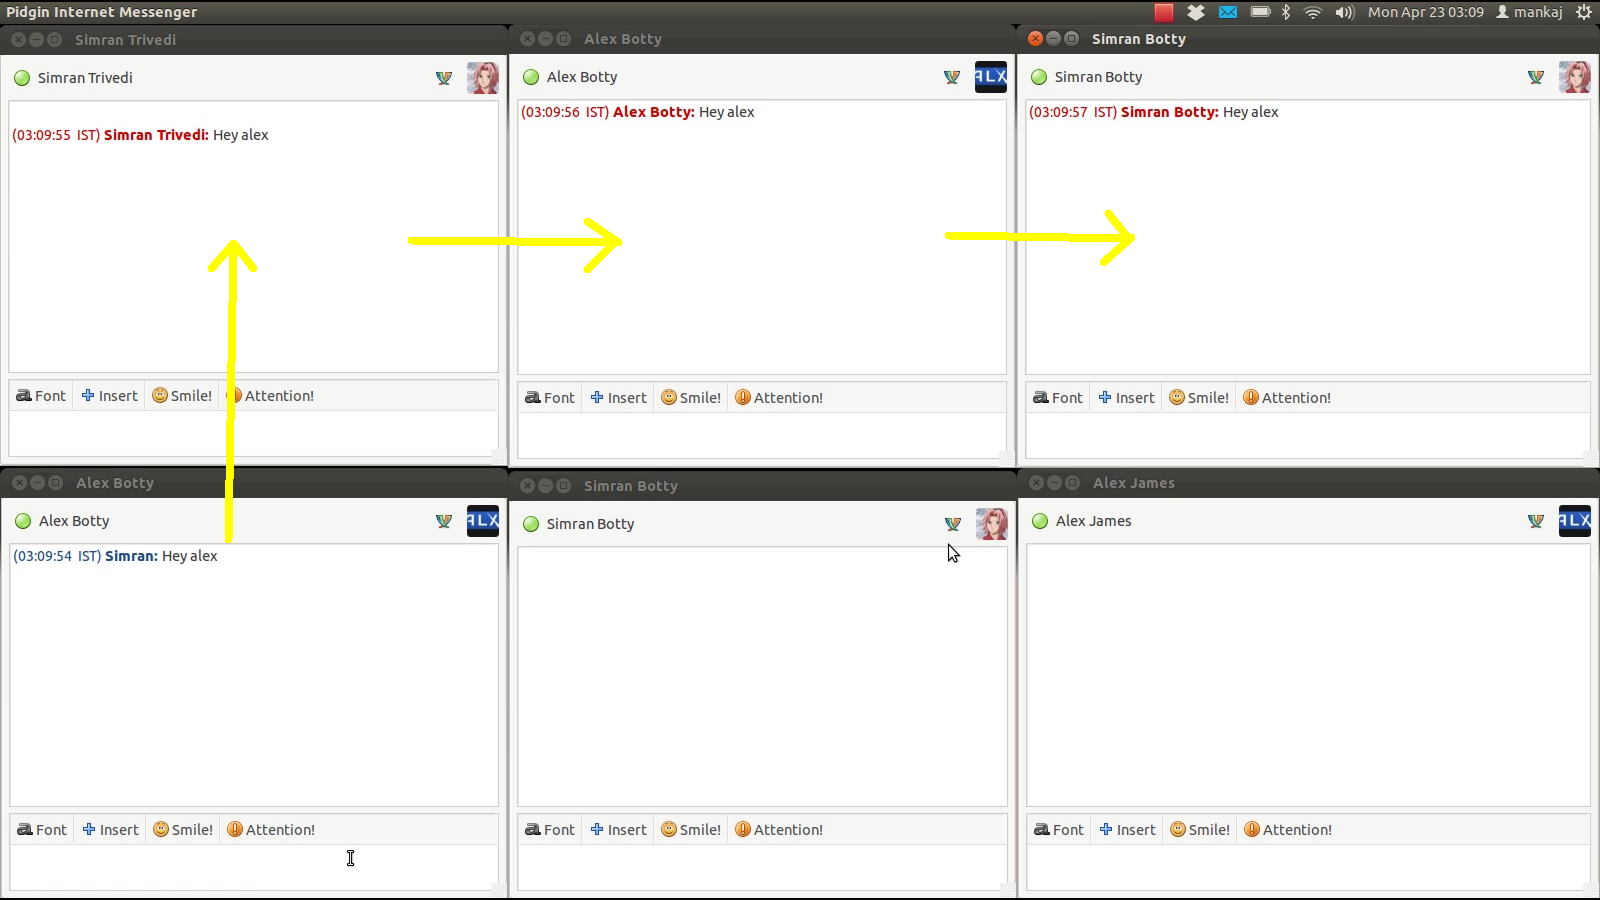
\includegraphics[scale=0.6, angle=90]{project/diagrams/attack1}
\caption{Facebook Chat Attack - 1}
\label{fig:attack1}
\end{figure}

\begin{figure}[H]
\centering
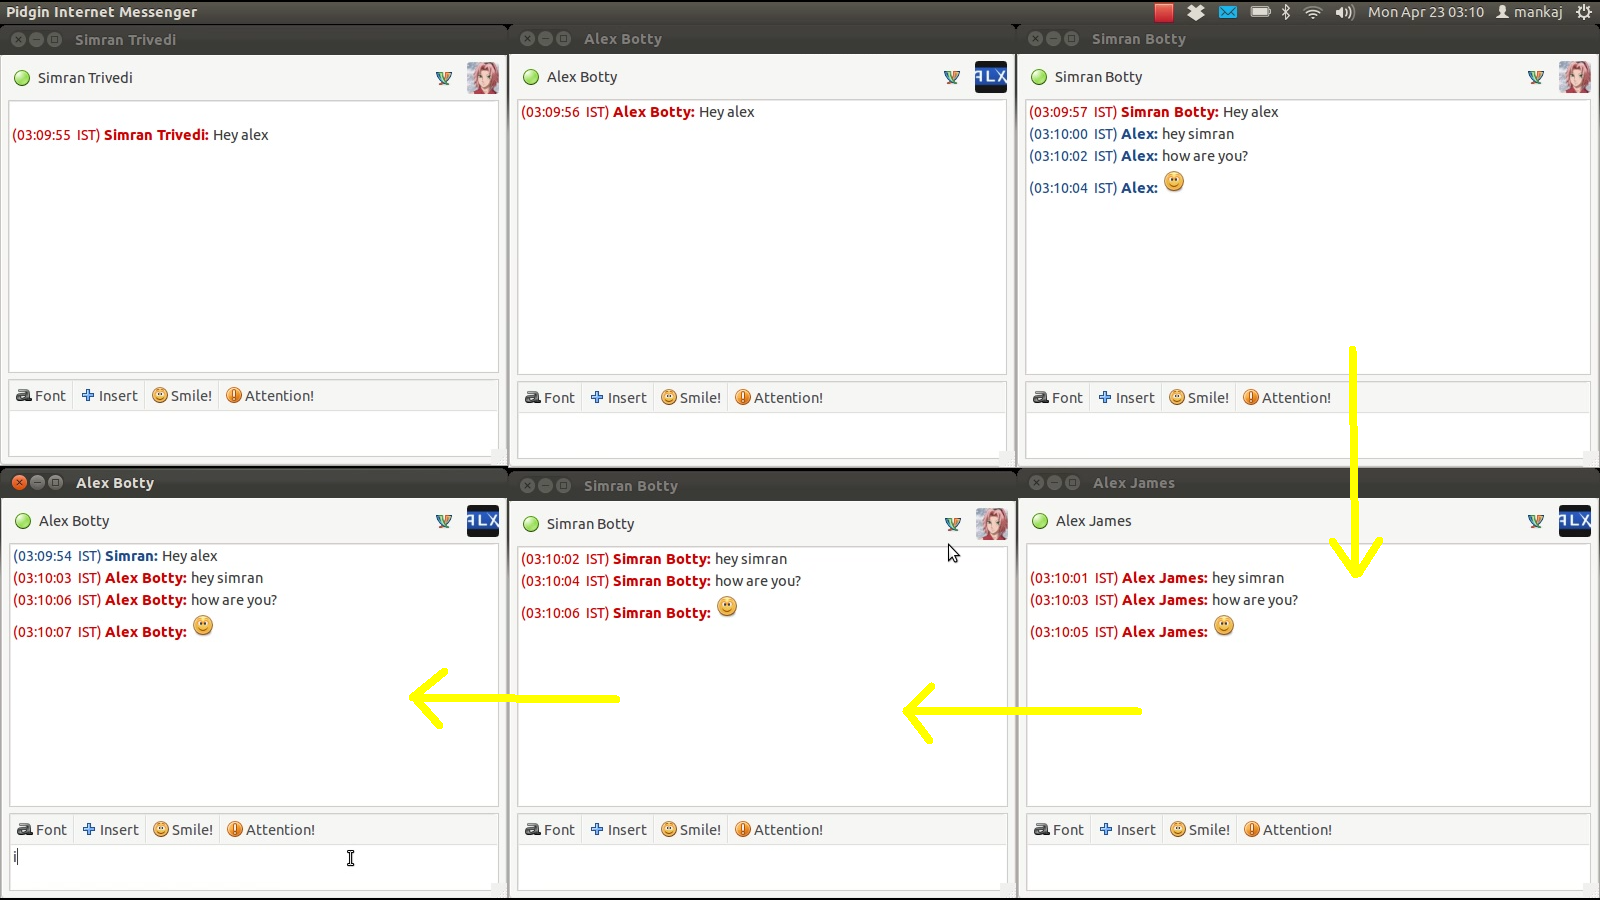
\includegraphics[scale=0.6, angle=90]{project/diagrams/attack2}
\caption{Facebook Chat Attack - 2}
\label{fig:attack1}
\end{figure}

\begin{figure}[H]
\centering
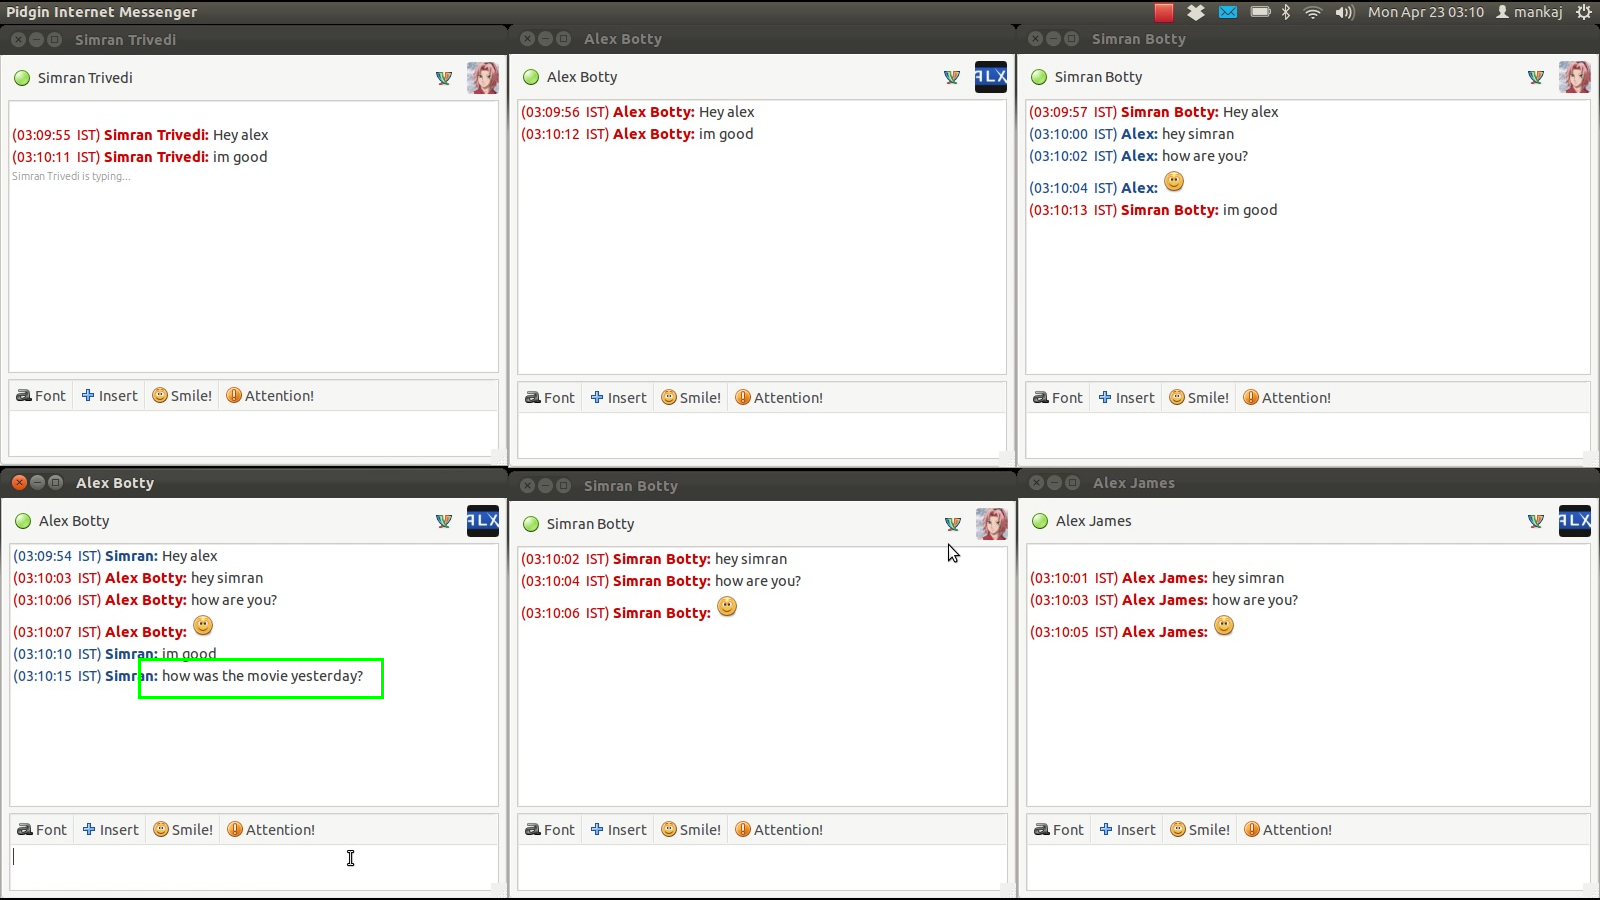
\includegraphics[scale=0.6, angle=90]{project/diagrams/attack3}
\caption{Facebook Chat Attack - 3}
\label{fig:attack1}
\end{figure}

\begin{figure}[H]
\centering
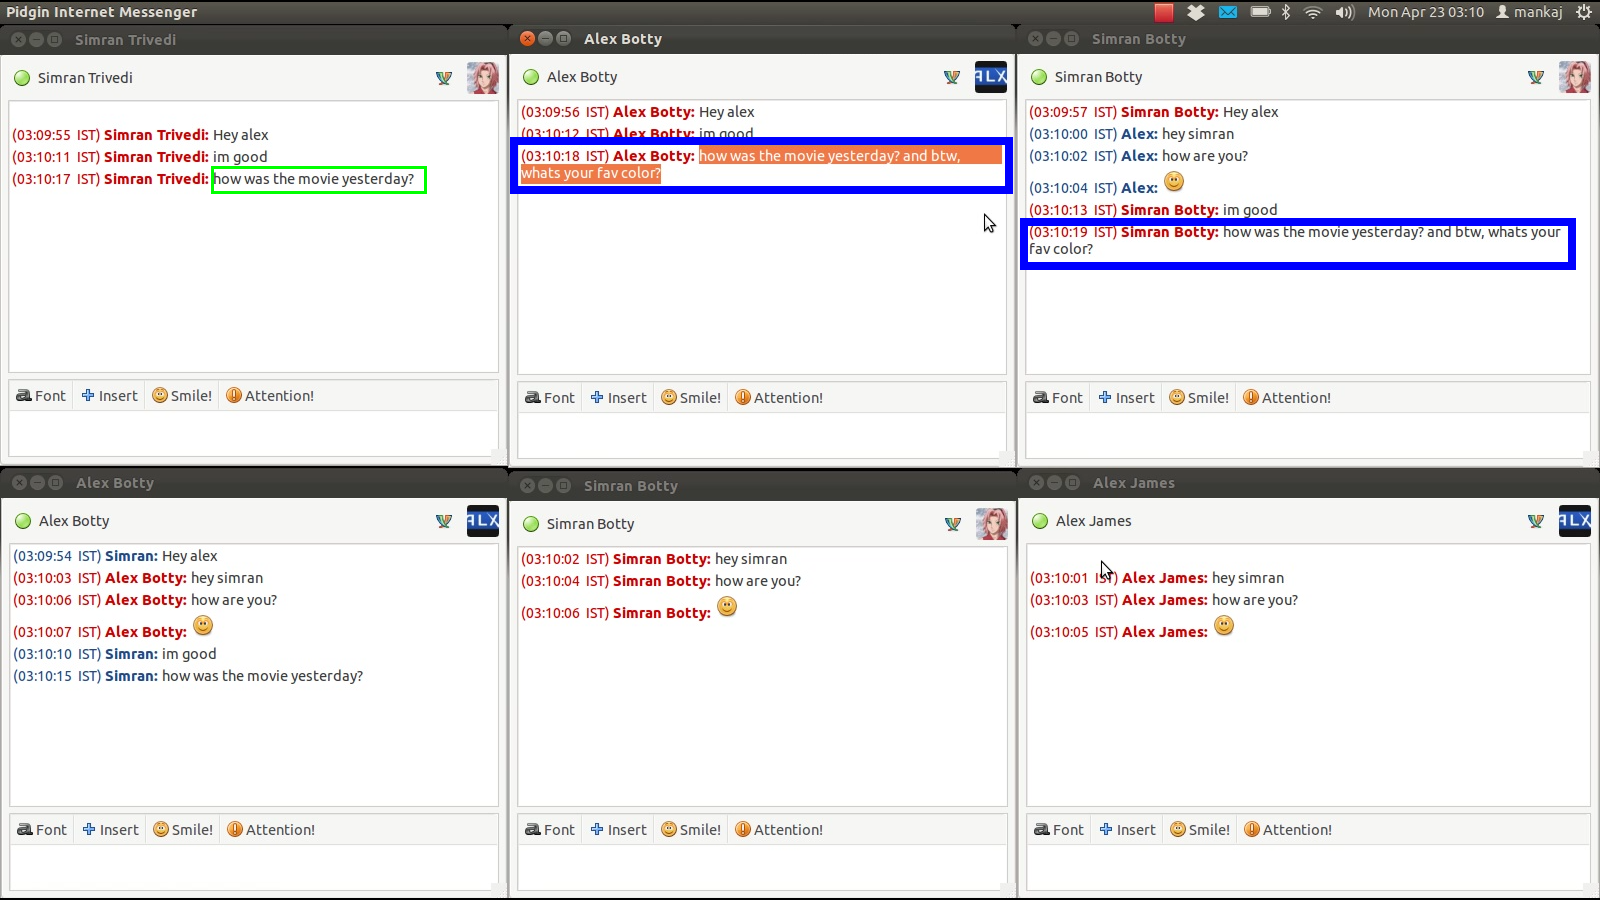
\includegraphics[scale=0.6, angle=90]{project/diagrams/attack4}
\caption{Facebook Chat Attack - 4}
\label{fig:attack1}
\end{figure}

\begin{figure}[H]
\centering
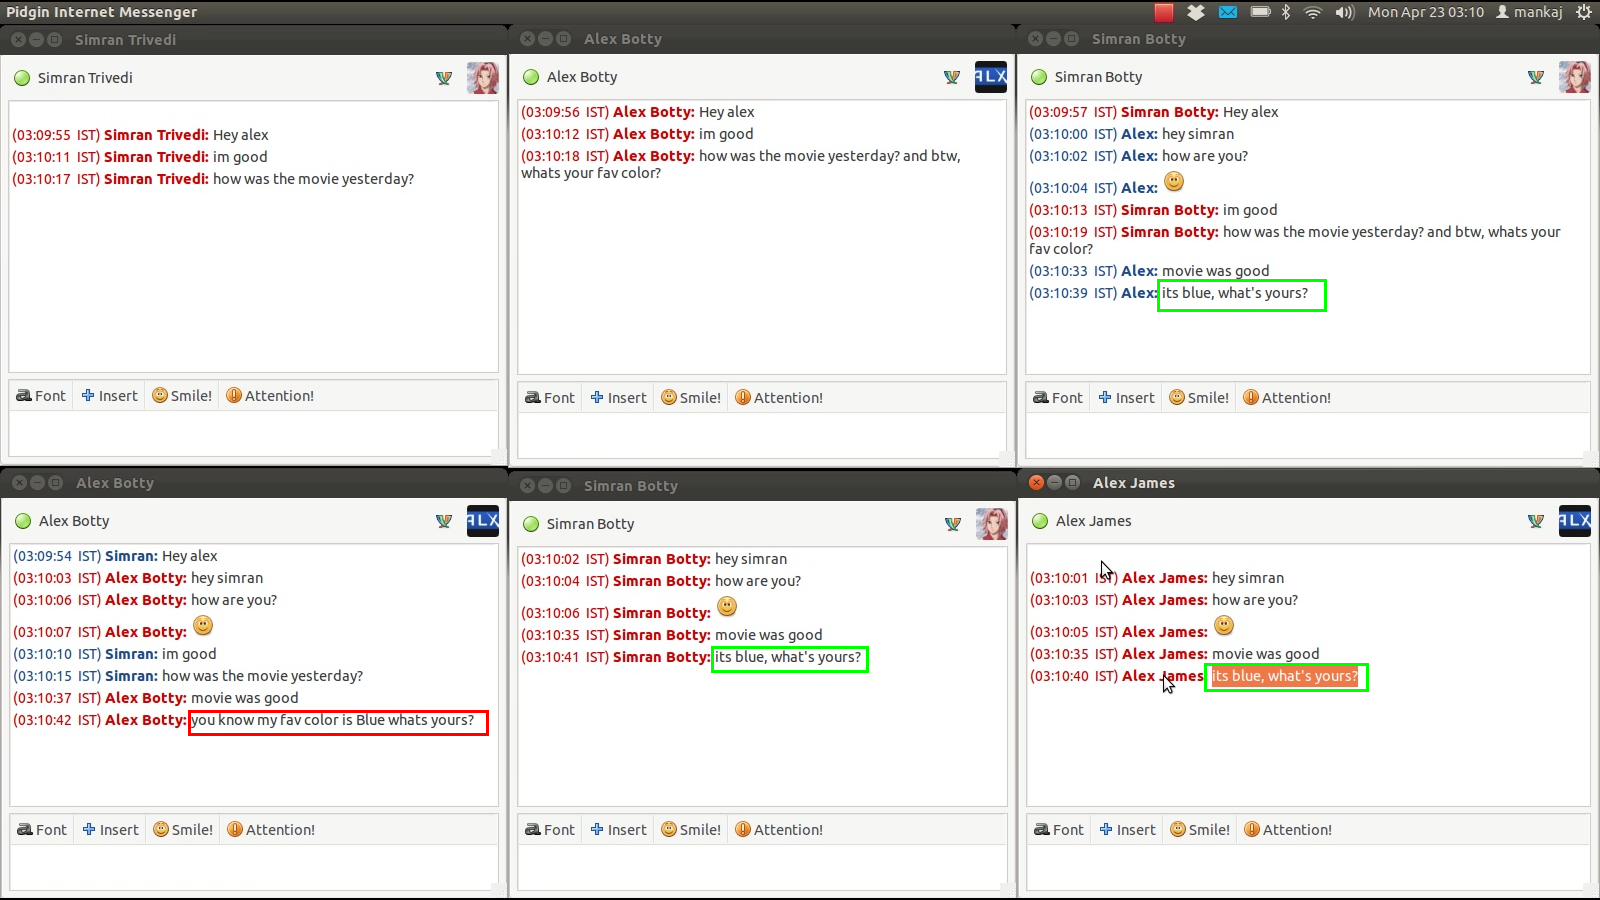
\includegraphics[scale=0.6, angle=90]{project/diagrams/attack5}
\caption{Facebook Chat Attack - 5}
\label{fig:attack1}
\end{figure}

\begin{figure}[H]
\centering
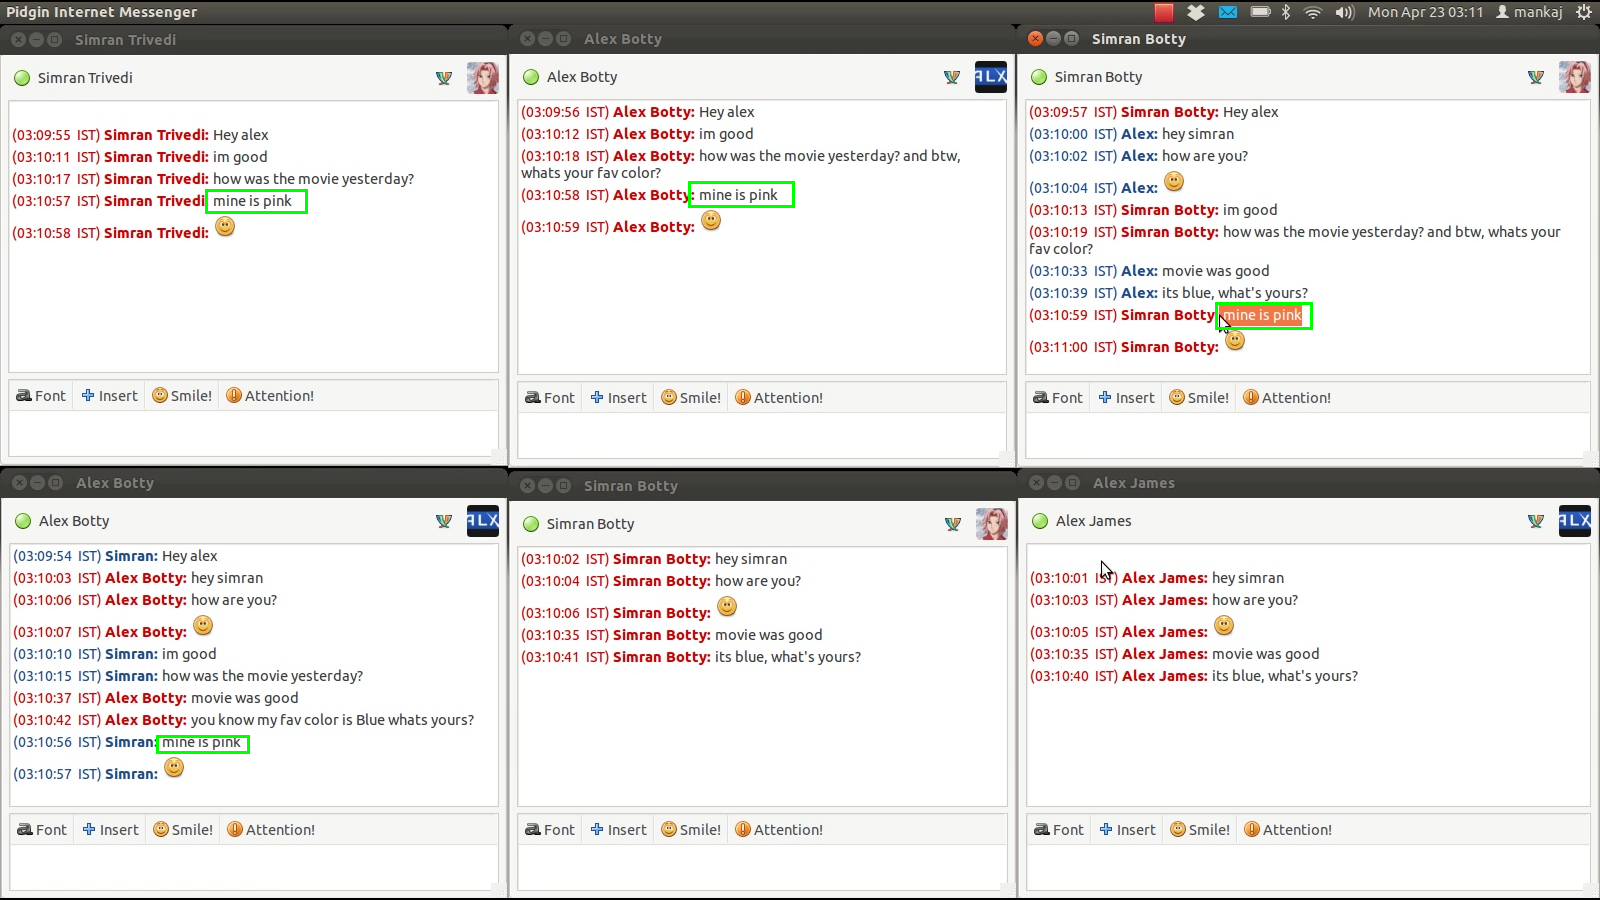
\includegraphics[scale=0.6, angle=90]{project/diagrams/attack6}
\caption{Facebook Chat Attack - 6}
\label{fig:attack1}
\end{figure}

